\documentclass[letterpaper,10pt]{article}

\usepackage{titling}
\usepackage{listings}
\usepackage{url}
\usepackage{setspace}
\usepackage{subfig}
\usepackage{sectsty}
\usepackage{pdfpages}
\usepackage{colortbl}
\usepackage{multirow}
\usepackage{multicol}
\usepackage{relsize}
\usepackage{amsmath}
\usepackage{wasysym}
\usepackage{fancyvrb}
\usepackage{amssymb}
\usepackage{ifsym}
\usepackage{amsmath,amssymb,amsthm,graphicx,xspace}
\usepackage[titlenotnumbered,noend,noline]{algorithm2e}
\usepackage[compact]{titlesec}
\usepackage{XCharter}
\usepackage[T1]{fontenc}
\usepackage{tikz}
\usetikzlibrary{arrows,automata,shapes,trees,matrix,chains,scopes,positioning,calc}
\tikzstyle{block} = [rectangle, draw, fill=blue!20, 
    text width=2.5em, text centered, rounded corners, minimum height=2em]
\tikzstyle{bw} = [rectangle, draw, fill=blue!20, 
    text width=4em, text centered, rounded corners, minimum height=2em]

\definecolor{namerow}{cmyk}{.40,.40,.40,.40}
\definecolor{namecol}{cmyk}{.40,.40,.40,.40}

\let\LaTeXtitle\title
\renewcommand{\title}[1]{\LaTeXtitle{\textsf{#1}}}


\newcommand{\handout}[5]{
  \noindent
  \begin{center}
  \framebox{
    \vbox{
      \hbox to 5.78in { {\bf ECE356: Database Systems } \hfill #2 }
      \vspace{4mm}
      \hbox to 5.78in { {\Large \hfill #4  \hfill} }
      \vspace{2mm}
      \hbox to 5.78in { {\em #3 \hfill} }
    }
  }
  \end{center}
  \vspace*{4mm}
}

\newcommand{\lecture}[3]{\handout{#1}{#2}{#3}{Lecture #1}}
\newcommand{\tuple}[1]{\ensuremath{\left\langle #1 \right\rangle}\xspace}

\addtolength{\oddsidemargin}{-1.000in}
\addtolength{\evensidemargin}{-0.500in}
\addtolength{\textwidth}{2.0in}
\addtolength{\topmargin}{-1.000in}
\addtolength{\textheight}{1.75in}
\addtolength{\parskip}{\baselineskip}
\setlength{\parindent}{0in}
\renewcommand{\baselinestretch}{1.5}
\newcommand{\term}{Winter 2018}

\singlespace


\begin{document}

\lecture{ 15 --- Query Processing }{\term}{Jeff Zarnett}

\section*{Query Processing}

Imagine you are given an assignment in a course and you are going to do it now. To get the assignment done, you will probably (1) figure out what exactly the assignment is asking you to do; (2) figure out how you are going to go it (e.g., must do part 1 first because part 2 depends on it...); and finally (3) do it! 

The procedure for the database server to carry out the query are the same~\cite{dsc}:

\begin{enumerate}
	\item Parsing and translation -- interpreting the SQL query in a form the computer can work with.
	\item Optimization -- figuring out how best to carry out the query.
	\item Evaluation -- execution of the query according to the plan just developed.
\end{enumerate}

To break these steps down into more detail, as in~\cite{fds}, the steps are a bit more like this. First, the scanner needs to figure out what are keywords and attribute names and relation names to figure out the text of the query. The parser will then check that it is valid SQL syntax. If so, then it will be validated to make sure that the attribute and relation names are valid inside the schema of the database being queried. Then this query is turned into a query tree or graph, which is used to devise the execution strategy. Then finally we can execute the query.

A quick visual summary of all the steps we are going to go through~\cite{dsc}:
\begin{center}
	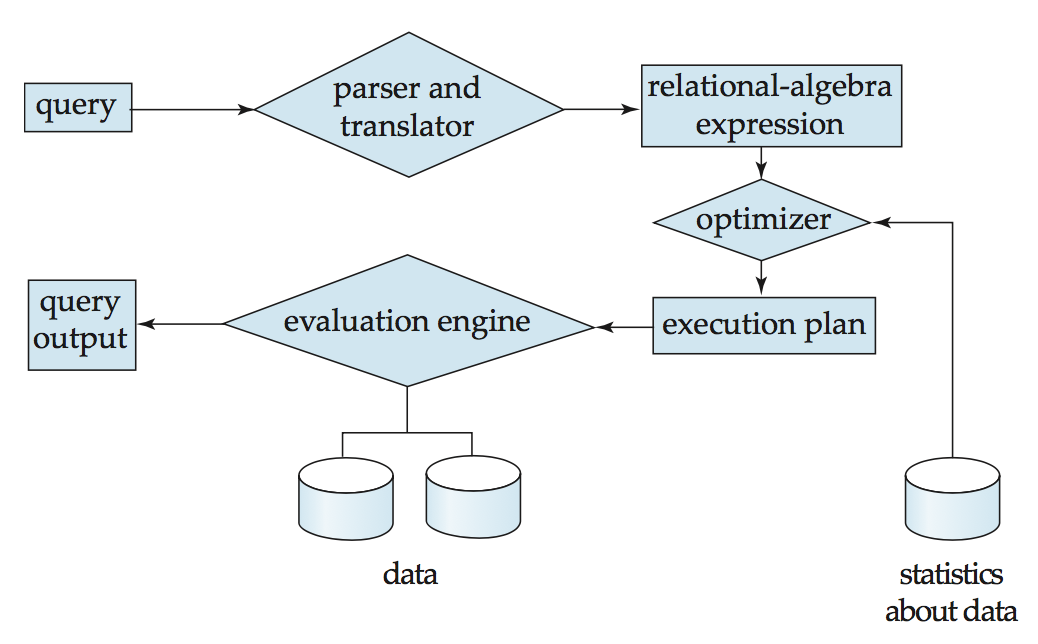
\includegraphics[width=0.5\textwidth]{images/query-processing-overview}
\end{center}

We will not spend time talking about the scanning, parsing, and verification steps of query processing. While they are all very important things and we need them, that is the sort of material that belongs in compiler textbooks and you may have already covered (or at least begun to cover) such material in a compilers course. In the meantime, if a query is syntactically invalid, or contains misspelled attributes, or something to that effect, we can't really do anything with it a query with an error is simply rejected and  goes no further through the process. We therefore will give them no further consideration.

Usually a query is expressed in SQL and that must then be translated into an equivalent relational algebra expression. Complex SQL queries are typically turned into \textit{query blocks}, which are translatable into relation algebra expressions. A query block has a single select-from-where expression, as well as related group-by and having clauses; nested queries are a separate query block~\cite{fds}.

A query like \texttt{SELECT salary FROM employee WHERE salary > 100000;} consists of one query block. The relational algebra for this expression is pretty easy to work out, and it gives us two possibilities. We can select all tuples where salary is more than 100~000 and then perform a projection of the salary field of that result (e.g., throw away the fields we do not need). The alternative is to do the projection of salary first and then perform the selection on the cut-down intermediate relation.

Suppose there is a subquery, like \texttt{SELECT name, street, city, province, postalCode FROM address WHERE id IN (SELECT addressID FROM employee WHERE department = 'Development');}. Then there are two query blocks, one for the subquery and one for the outer query. If there are multiple query blocks, then they do not have to follow the same strategy; they can be optimized separately if desired. 

The relational algebra is not quite enough to actually carry out the operation. What we need instead is a \textit{query execution plan}\footnote{\url{https://www.youtube.com/watch?v=fQk_832EAx4}}. To build that up, each step of the plan needs annotations that specify how to evaluate the operation, including information such as what algorithm or what index to use. An algebraic operation with the associated annotations about how to get it done is called an \textit{evaluation primitive}. The sequence of these primitives forms the plan, that is, how exactly to execute the query~\cite{dsc}. 

If there are multiple possible way to carry out the plan, which there very often are, then the system will need to make some assessment about which plan is the best. It is not expected that users will write optimal queries; instead the database server should choose the best approach via \textit{query optimization}. Optimization is perhaps the wrong name for this because we are not choosing the optimal approach; instead we will make some estimates about the query plans and try to choose the one that is most likely to be best. The subject of query optimization is something we will touch on now, but also come back to when we have more understanding.

\subsection*{Measures of Query Cost}

If you are asked to drive a car from point A to point B and there are multiple routes, you can evaluate your choices. To do so you need to break it down into different sections, such as drive along University Avenue, then get on Highway 85, then merge onto 401... Each segment has a length and a speed, such as knowing that you will drive 4 km along University Avenue and it is signed at 50 km/h (although with red lights and traffic and whatnot the actual average speed may be more like 30 km/h). By combining all of the segments, you get an estimate of how long that particular route will take. If you do this for all routes, you can see which route is the best. 

Of course, it may turn out that real life gets in the way: if there is a crash on the highway, traffic really sucks and your decision that taking this particular route would be fastest turns out to be wrong. Short of being able to see into the future, this is more or less inevitable: estimates are just informed opinions and things may be worse (or better) than expected. 

Where does the time go in executing a query? The biggest component is most likely loading blocks from disk, considering how slow the disk operations are. Although we can improve this via use of SSDs, many large databases still use hard disk drives. CPU speeds are pretty fast, to the point even where memory accesses seem slow from the perspective of the CPU. So, no matter what we do, disk accesses likely account for far more of the time than CPU computation. In reality, CPU time is a nonzero part of query optimization, but we will ignore this (as does~\cite{dsc}) for simplicity's sake and use only the disk accesses to assess cost.

The number of block transfers (data moved in and out of memory) and the number of disk seeks (repositioning where on the disk we are reading from) are the important measures of interest here. SSDs have no seek time and have faster transfer speeds, but the number of block transfers is still relevant. To compute the estimate of how long we think it will take to perform an operation, the formula is $b \times t_{T} + S \times t_{s}$ where $b$ is the number of block transfers, $t_{T}$ is the time to transfer, $S$ is the number of seeks, and $t_{s}$ the time it takes to seek~\cite{dsc}. For a hard drive, transfer times are on the order of 0.1~ms and seek times are about 4~ms.

We will follow the estimating strategy in~\cite{dsc} which comes with a few caveats, explained in this paragraph. Sometimes writes can be twice as expensive as reads. This is because the disk subsystem may read back the written data to check that the write succeeded, but we will assume that does not happen here. Similarly, at this first level we are not including the amount of time it takes to write a final result back (that depends on the query... a select, for example, may not need it, where an update will). That cost would be accounted for separately. And the asterisk here is that the size of memory makes a big difference -- if the buffer is large enough that all of the database fits in it, then disk reads are almost never needed. We will imagine the worst case scenario, that is, only one block per relation can be in memory at a time. If we are ``wrong'' and the data we need is already in memory, the actual cost is less than the estimated cost (which is better than the reverse). 

The estimates calculate only the amount of work that we think it will take to complete the operation. Unfortunately, there are several factors that will potentially affect the actual wall-clock time it takes to carry out the plan:

\begin{itemize}
	\item How busy the system is -- if there are multiple concurrent operations then any particular operation may be queued or blocked or otherwise not able to proceed immediately, leading to a longer time to completion.
	\item What is in the buffer -- if partial data is in the buffer that will speed up completion of the operation since some planned disk operations can be skipped.
	\item Data layout -- if the data is packed well on disk then we need to do fewer seek operations (or shorter ones, perhaps); likewise, if the data is distributed over multiple physical disks we can sometimes do some reads in parallel, but it's hard to know exactly how much parallelization is possible.
\end{itemize}

You can probably think of various other factors that will affect the time it takes to execute the query in reality. The estimate is just an educated guess that we will use to plan how to do the work; it's not a promise of exactly how long it will take.

Note also that the lowest cost approach is not necessarily the fastest. Sometimes we can go faster by using more resources, but the approach the database often takes is the lowest cost (specifically, fewest disk reads). Recalling the earlier driving analogy, you can think of this as perhaps driving a longer route that involves more highway driving and therefore less time, even if it means more fuel consumption due to the increased distance and speed. When driving, we generally prefer to choose the lowest time estimate, but there are also people (``hypermilers'') who are really obsessed with getting maximum fuel economy... and the database is one of those people!

\subsection*{Select Operation}
The first example we will see about estimating cost is how to do a select operation. We will consider a lot of possibilities, some of which are obviously sub-optimal. We should consider all options (this is good advice in science in general, consider all possibilities, even the null hypothesis) even if we are pretty sure one of them is going to be terrible... we might be surprised. In other cases, a seemingly-terrible algorithm is our last resort, such as if we have to find something that has no index, we perform the painstaking linear search approach. The strategies considered in this section come from~\cite{dsc}.

We will assume that we have a select-from-where condition to be evaluated on a single relation.  The relation itself is stored in a single file and this file contains only records of that single relation. 

\subsubsection*{General Selection}

The first approach is general and really needs no introduction.

\paragraph{Select Strategy 1A: Linear Search.} The linear search is exactly what it sounds like: scan each file block from beginning to end to see if the selection condition is satisfied. We can assume the file is stored efficiently so we have only one seek to start reading the file, and then the transfer time for each block. Thus there is one seek plus one transfer for each block of the file and the cost estimate is $t_{s} + n \times t_{T}$ where $n$ is the number of blocks in the file (worst case scenario). 

As mentioned earlier, linear search is probably inefficient if we have any other alternative. However, if there is no index and the file is not ordered on the search predicate, we may not have any other choice. But as a last resort, we can be sure this will work.

\subsubsection*{Selection with Equality}

We would much prefer, if we can, to use an index of some sort. If we have that, we can access a lot fewer records than we would otherwise need to. The following group of strategies are applicable when the where condition contains an equality test, e.g., ``province equals Ontario''.

\paragraph{Select Strategy 1B: Binary Search}
Binary search is also exactly what we are pretty well familiar with. If the file is ordered on something other than the primary key, and this is the where condition, we can search using a binary search algorithm. Binary search would then mean we can significantly reduce the number of blocks we need. But we will assume generally from here that we will look at B$^{+}$ trees.

\paragraph{Select Strategy 2: Primary Index, Equality on Key}
If the select's where clause specifies equality on a primary index, i.e., the way the file is organized, it is very efficient. We will have to traverse the tree to get to the leaf containing the pointer to the record. That means one seek and one transfer for each of the levels of the tree. Then finally we access the data directly, which is another seek and another transfer. Thus the cost estimate is $(h_{i} + 1) \times (t_{s} + t_{T})$ where $h_{i}$ is the height of the index B$^{+}$ tree.

\paragraph{Select Strategy 3: Primary Index, Equality on Non-Key}
If the primary index for the file is a non-key (non-unique) field then instead of getting one record we may get multiple records. Of course, this should be a rare occurrence because the primary index being a non-key is not recommended. But if such a query has to be carried out we need an estimate of the cost. The multiple records will be consecutive, because it is the primary index. Thus the cost will be $h_{i} \times (t_{s} + t_{T}) + b \times t_{T}$ where in this case $b$ is the number of block containing the target search key. Because the blocks with the actual data are stored sequentially we don't need to check the index again for the next ones, nor do we need to seek to them.

Estimating $b$ can be somewhat difficult. If we know there are two matches they could be in the same block or in two different blocks. We may need to guess about how many match.

\paragraph{Select Strategy 4: Secondary Index, Equality}
If the secondary index is on a unique field, then the cost estimate is the same as strategy 2:  $(h_{i} + 1) \times (t_{s} + t_{T})$.

If the key is not unique then the cost is higher. Unlike strategy 3, we cannot rely on the fact that the records are consecutive. In fact, they are almost certainly not. We make the opposite assumption, that each record requires a seek and a transfer of a new block. This the estimate is $(h_{i} + k) \times (t_{s} + t_{T})$ where $k$ is the number of records matching the condition.

As with $b$ in strategy 3, estimating the value of $k$ is probably difficult. In the worst case it means reading from every block of the file because there is (at least) one matching record in each block.

\subsubsection*{Selection with Comparison}

Until this point we just handled an equality condition, where we looked for an exact match. A comparison is more complex. We can still use the linear search approach, if we must, but if we have an index we may still prefer to use that. We will continue to assume that the file index is organized in a B$^{+}$ tree.

\paragraph{Select Strategy 5: Primary Index, Comparison}
Suppose our desired search value is $x$. If the attribute being compared is $A$, then our possibilities are (1) $A > x$ or $A \geq x$, (2) $A < x$ or $A \leq x$.

For the first case, we use the tree to go to the first tuple where $A = x$ or $A > v$ respectively. Then we do a file scan from start to the end of the file. In that case, our cost estimates are like those of strategy 3.

For the second case, we start at the beginning of the file and go until the first tuple with $A = x$ or $A > x$ respectively. This is more or less a linear scan that may end early. When doing this comparison, the index contributed absolutely nothing (although we could look at it, one imagines, to refine the estimate of where the reading will end).

\paragraph*{Select Strategy 6: Secondary Index, Comparison}
This case very much resembles the case of strategy 4, equality on a non-key field. Fetching the actual data is a pain, of course. If the number of records to be fetched is large, because of all the jumping back and forth, it might actually be worse than simply performing a linear search.  It depends on the value of $k$, how many records will match. 

\subsubsection*{Complex Selection}

The previous strategies, aside from linear search, assumed the predicate had one clause. Before we start, a quick review of the ideas of conjunction, disjunction, and negation (from basic algebra) from~\cite{dsc}:

A conjunctive selection involves the logical and operation. In relational algebra, the selection operation is written $\sigma_{\theta_{1}} \wedge \sigma_{\theta_{2}} \wedge ... \wedge \sigma_{\theta _{n}}( r )$. This describes selection of all the tuples that match all of the predicate clauses.

A disjunctive selection involves the logical or operation. In relational algebra, the selection operation is written $\sigma_{\theta_{1}} \vee \sigma_{\theta_{2}} \vee ... \vee \sigma_{\theta _{n}}( r )$. This describes selection of all the tuples that match one or more of the predicate clauses. This is equivalent to the union of all the tuples matching each of the individual $\theta_{i}$ conditions.

A negation selection $\sigma_{\neg \theta}(r)$ is the set of all tuples of $r$ for which the condition $\theta$ evaluates to false. 

\paragraph{Select Strategy 7: Conjunction, One Index}
Since we need to satisfy all conditions, we will first find all records that satisfy one of the simple conditions, and then throw away any of the retrieved that do not match the remaining conditions. One of the previous strategies (2 through 6) will suffice, and the cost is pretty much determined by which of those strategies is used. We would take estimates for each strategy and choose the one with the lowest expected cost.

Ah, but which simple condition do we choose? If only one has an index, then we use the one index. That was easy. If there are multiple choices, ideally we choose the most restrictive -- the one that will match the fewest tuples. That would then result in less loading of tuples that we are just going to throw away. This is another case where, as you might imagine, it is not immediately clear how to know which condition matches the fewest tuples. There are approaches for making good decisions, which will be a topic of future discussion. 

\paragraph{Select Strategy 8: Conjunction, Composite Index}
Recall from the discussion of indexing that a composite index is one that is on multiple attributes. If the selection has multiple simple conditions, a subset of which exist in a composite index on the relation, that is very helpful. Then we can use the index directly. If the complex where predicate is exactly equal to the composite index, we will be using one of strategies 2, 3, or 4. If there are some conditions that form the composite index and others that do not, our strategy looks more like strategy 7. Again, take some estimates of each possible execution plan to decide what to do.

\paragraph{Select Strategy 9: Conjunction, Intersection}
Another way we could do the conjunction would be to look at the record pointers. We get a list of record pointers for each simple condition that has an index and compute the intersection of these. If there are any conditions on attributes without an index, then we must further look through the results to throw away those records that don't meet all conditions.

The cost here is the sum of the cost of looking through each index, plus the cost of loading the records after the intersection is computed. In theory we can reduce the amount of work necessary by simply sorting the pointers before we retrieve data, which would make the disk reads closer to sequential and minimize the amount of seeking that needs to be done.

\paragraph{Select Strategy 10: Disjunction, Union}
Much like the conjunction strategy, we get a list of record pointers for each of the conditions where there is an index. Instead of computing the intersection, we find the union (no duplicates) of these pointers. Again, sorting may make the disk reads closer and speed things along significantly.

If there is at least one condition that does not have an index, then it is makes sense to just linear scan since we are going to have to do that anyway.

\paragraph{Select Strategy 11: Negation}
The authors in~\cite{dsc}, as they are known to do, leave the explanation of this strategy ``as an exercise'' for the reader.  Although one can, of course, do a linear scan to find those that, unlike usual, do NOT meet the given conditions, what can one do? 

If we have an index on the field that might help: we can evaluate the index and decide which records match the not condition, and only load those. As the last resort, the linear search approach will be necessary.



\bibliographystyle{alphaurl}
\bibliography{356}


\end{document}
